
\begin{frame}
 \frametitle{Stochastic Point of View}
 Actions $\rightarrow$ Markov Equations and are well posed with IC and BCs:
    \[
\frac{\partial \Phi(z_c,t)}{\partial t} = \sum_j  a_j(z_o,t)\Phi(z_o,t) -\sum_k a_k(z_c,t)\Phi(z_c,t)
\]
\begin{columns}
 \column{0.5\textwidth}
 \textcolor{blue}{Multivariate Bernoulli Distribution}
 \begin{itemize}
  \item Discrete
  \item Permutable
  \item Interconnected
 \end{itemize}
 Stochastic Simulation (PINT)\\
 Numerical Techniques
 \column{0.40\textwidth}
  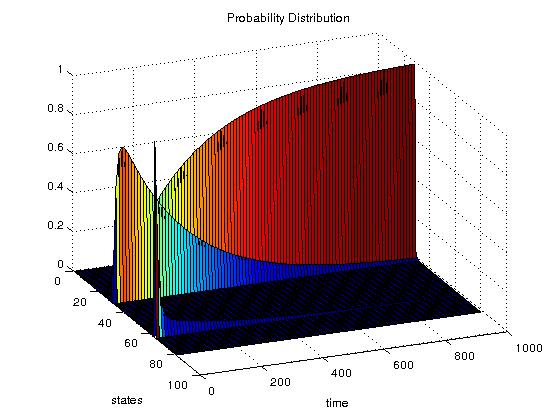
\includegraphics[trim=0mm 0mm -50mm 0mm, width=70mm,height=50mm]{./figures/MH_probab_plot.jpg}
\column{0.1\textwidth}
\hfill
\end{columns}

\end{frame}


\begin{frame}
 \frametitle{Numerical Techniques}
 \textcolor{blue}{Now}: \textcolor{red}{Proper Generalized Decomposition}
 \begin{itemize}
 \item Model Reduction technique similar to SVD
  \item $\Phi(z_c,t) \approx \sum\limits^{M}_{j=1}A_j(a) B_j(b)  C_j(c)\cdots T_j(t)$
  \item $N^{N_{sp}}\rightarrow M\left( N\times N_{sp} \right)$
  \item Easy transition to parametric models
 \end{itemize}
 \vspace{1cm}
\textcolor{blue}{Future}: \textcolor{red}{Moment Closure/ PGD Hybrids}
\begin{itemize}
 \item Use static analysis to determine required Cooperative Sorts
 \item Combine initial solution of PGD to Moment Closure Scheme
 \item Potential pitfalls in scalability, production of equations
\end{itemize}


\end{frame}
